\documentclass[11pt, a4paper, twosided, openright]{book}
\usepackage[papersize={216mm,303mm},
    layout=a4paper,
    layouthoffset=3mm,
    layoutvoffset=3mm,
    bindingoffset=0.5cm, %1cm,
    top=1.5cm, bottom=1.5cm,
    left=1.5cm, right=1.5cm,
    headheight=12pt,
    includehead, includefoot,
    heightrounded]{geometry}
\usepackage[hidelinks]{hyperref}
\usepackage{emptypage}

\usepackage{tgcursor}
\renewcommand*\familydefault{\ttdefault}
\usepackage[british]{babel}
\selectlanguage{british}
\usepackage[useregional]{datetime2}
\DTMdefboolkey{en-GB}{showdayofmonth}[false]{}
\usepackage{fontawesome5}
\usepackage[utf8]{inputenc}
\usepackage[T1]{fontenc}
\setlength{\parindent}{0cm}
\setlength{\parskip}{0cm}
\extrafloats{100}

\usepackage{graphicx}

\def\textpagetopmargin{4cm}
\def\textpageparscpacing{3cm}

\newcommand{\chapterpage}[1]{
  \cleardoublepage{\thispagestyle{empty}}

  \vspace*{10cm}
  \begin{minipage}{\textwidth}
    \centering
    #1
  \end{minipage}

  \cleardoublepage{}
}

\newcommand{\pagerileri}[3]{
    \clearpage
    \par\vspace*{\textpagetopmargin}\hfill
    \begin{minipage}{0.7\textwidth}
        \raggedleft\huge #1
    \end{minipage}
    \par\vspace{\textpageparscpacing}
    \begin{minipage}{0.7\textwidth}
        \raggedright #2
    \end{minipage}\hfill
    \par\vspace{\textpageparscpacing}\hfill
    \begin{minipage}{0.7\textwidth}
        \raggedleft #3
    \end{minipage}
}

\newcommand{\pagelerile}[3]{
    \clearpage
    \par\vspace*{\textpagetopmargin}
    \begin{minipage}{0.7\textwidth}
        \raggedright\huge #1
    \end{minipage}\hfill
    \par\vspace{\textpageparscpacing}\hfill
    \begin{minipage}{0.7\textwidth}
        \raggedleft #2
    \end{minipage}
    \par\vspace{\textpageparscpacing}
    \begin{minipage}{0.7\textwidth}
        \raggedright #3
    \end{minipage}\hfill
}
\makeatletter

    \def\@publishing{First}
    \def\@printing{First}
    \def\@zinenumber{Zine 1}
    \def\@zinetitle{Rosteig}
    \def\@zinesubtitle{Endless forests and tranquility}

    \author{Arthur Van de Wiele}
    \title{\@zinenumber\ $\cdot$ \@zinetitle\ $\cdot$ \@zinesubtitle}
    \date{\today}

\makeatother



\begin{document}

\thispagestyle{empty}

\makeatletter

  \vspace*{7cm}

  \begin{minipage}[t][][b]{0.80\textwidth}
    \raggedright
    \vspace{2cm}
    \setlength{\parskip}{1em}
    \includegraphics[height=3cm]{template/marmot.jpg}\par
    \vspace{1cm}
    \@publishing\ Edition $\cdot$ \@printing\ Print $\cdot$ \@date
  
    Title: \@title\newline
    Author: \@author\newline
    Photography: \@author\newline
    Publisher: N/A\newline
    Editor: \@author\newline
    Design and Layout: \@author\newline
    Distribution: N/A

    {\tiny \faHandPointer[regular] That's a lot of me...}
  
    Copyright \copyright~by \@author. All right reserved.
  
    ISBN: N/A
  
    {\bfseries All rights reserved}\newline
    No part of this work may be reproduced in any form or by any means without permission in writing from the Author or Publisher.
  \end{minipage}
    
\makeatother


\makeatletter
    \chapterpage{
    {\par\huge\bfseries \@zinetitle}
    \vspace{1cm}
    {\par\huge \@zinesubtitle}
    }
\makeatother

\pagerileri{
    Foreword%
}{
    I must have travelled these paths a hundred times by now, yet their magic never fades. I will never get tired of the vibrant colours of Alsatian houses nor of the gentle murmur of the wind weaving through the treetops above this serene and protected valley. I would like to show you my home away from home, where the noise of the world quiets down and nature is all there is to see and hear.%
}{
    Nestled in the heart of the Northern Vosges Regional Natural Park, Rosteig is a small French village where time seems to stand still, surrounded by endless forests and steeped in tranquility. It is where I get away from the bustling city of Munich where\\ I otherwise reside, and I wish for these\\ photographs to carry some of the beauty\\ and peace I found here.%
}

\cleardoublepage


    \begin{figure}
    \centering
    \phantomsection\label{img:images/001.jpg}
    \includegraphics[height=\textheight, width=160mm, keepaspectratio]{images/001.jpg}%
    \end{figure}
    
    \begin{figure}
    \centering
    \phantomsection\label{img:images/002.jpg}
    \includegraphics[height=\textheight, width=160mm, keepaspectratio]{images/002.jpg}%
    \end{figure}
    
    \begin{figure}
    \centering
    \phantomsection\label{img:images/003.jpg}
    \includegraphics[height=\textheight, width=160mm, keepaspectratio]{images/003.jpg}%
    \end{figure}
    
    \begin{figure}
    \centering
    \phantomsection\label{img:images/004.jpg}
    \includegraphics[height=\textheight, width=160mm, keepaspectratio]{images/004.jpg}%
    \end{figure}
    
    \begin{figure}
    \centering
    \phantomsection\label{img:images/005.jpg}
    \includegraphics[height=\textheight, width=160mm, keepaspectratio]{images/005.jpg}%
    \end{figure}
    

\chapterpage{\huge Index}

\pagerileri{
    I'd rather be outside, shooting, than inside, editing.%
}{
    I do study the work of other photographers to understand how I can improve my photography. So I decided to include an index of all the pictures in this Zine with information about the gear I used, the camera settings, and so on. The pictures in this collection were shot with digital cameras. For the most part, I shoot in aperture priority with manual exposure compensation, and custom auto-ISO settings aimed at maintaining a shutter speed no lower than 1/125th or 1/250th of a second depending on the lens and type of situation I am in. I shoot in either auto-white balance with some shifts in the colour cast, or fully manual (e.g. 5700K for mid-summer daylight).%
}{
    Every photograph here was shot directly in JPEG, using custom settings to get the images as close to the final look as possible. In post, I sparsely adjust colours, contrast and white balance to harmonize pictures across a collection, and might need to crop ever so slightly if something close to the frame bothers me too much. But for the most part, the images are as close as possible to\\ how they were shot.%
}

% File is automatically generated. Edits will be overwritten.


\begin{minipage}{0.25\textwidth}
  \includegraphics[width=43mm, keepaspectratio]{001.jpg}
\end{minipage}
\hfill
\begin{minipage}{0.70\textwidth}
  \raggedright
  \par \raisebox{-0.1\height}{\faImage[regular]}~\textbf{Photo \#1} $\cdot$ Page~\pageref{img:001.jpg} $\cdot$ February 2024
  \par Fujifilm X-E3
  \par  
  \par No Aperture Information $\cdot$ 1/170 sec $\cdot$ ISO 400
  \par Auto $\cdot$ Matrix Metering +1 and 1/3 stop
\end{minipage}
\vspace{0.5cm}

\begin{minipage}{0.25\textwidth}
  \includegraphics[width=43mm, keepaspectratio]{002.jpg}
\end{minipage}
\hfill
\begin{minipage}{0.70\textwidth}
  \raggedright
  \par \raisebox{-0.1\height}{\faImage[regular]}~\textbf{Photo \#2} $\cdot$ Page~\pageref{img:002.jpg} $\cdot$ September 2024
  \par Fujifilm X-T50
  \par Minolta MD 35-70mm f/3.5 + K\&F Concept MD-FX Adapter
  \par No Aperture Information $\cdot$ 1/250 sec $\cdot$ ISO 1600
  \par Auto $\cdot$ Matrix Metering +1 stop
\end{minipage}
\vspace{0.5cm}

\begin{minipage}{0.25\textwidth}
  \includegraphics[width=43mm, keepaspectratio]{003.jpg}
\end{minipage}
\hfill
\begin{minipage}{0.70\textwidth}
  \raggedright
  \par \raisebox{-0.1\height}{\faImage[regular]}~\textbf{Photo \#3} $\cdot$ Page~\pageref{img:003.jpg} $\cdot$ August 2024
  \par Fujifilm X-T50
  \par Fujifilm XF 35mm f/2.0 R WR
  \par f/2.0 $\cdot$ 1/2700 sec $\cdot$ ISO 400
  \par Auto $\cdot$ Matrix Metering +1 and 1/3 stop
\end{minipage}
\vspace{0.5cm}

\begin{minipage}{0.25\textwidth}
  \includegraphics[width=43mm, keepaspectratio]{004.jpg}
\end{minipage}
\hfill
\begin{minipage}{0.70\textwidth}
  \raggedright
  \par \raisebox{-0.1\height}{\faImage[regular]}~\textbf{Photo \#4} $\cdot$ Page~\pageref{img:004.jpg} $\cdot$ May 2024
  \par Fujifilm X-E3
  \par  
  \par No Aperture Information $\cdot$ 1/200 sec $\cdot$ ISO 400
  \par Auto $\cdot$ Matrix Metering +1 stop
\end{minipage}
\vspace{0.5cm}

\begin{minipage}{0.25\textwidth}
  \includegraphics[width=43mm, keepaspectratio]{005.jpg}
\end{minipage}
\hfill
\begin{minipage}{0.70\textwidth}
  \raggedright
  \par \raisebox{-0.1\height}{\faImage[regular]}~\textbf{Photo \#5} $\cdot$ Page~\pageref{img:005.jpg} $\cdot$ August 2024
  \par Fujifilm X-T50
  \par Fujifilm XF 35mm f/2.0 R WR
  \par f/2.0 $\cdot$ 1/3000 sec $\cdot$ ISO 400
  \par Auto $\cdot$ Matrix Metering +1 and 1/3 stop
\end{minipage}
\vspace{0.5cm}

\begin{minipage}{0.25\textwidth}
  \includegraphics[width=43mm, keepaspectratio]{006.jpg}
\end{minipage}
\hfill
\begin{minipage}{0.70\textwidth}
  \raggedright
  \par \raisebox{-0.1\height}{\faImage[regular]}~\textbf{Photo \#6} $\cdot$ Page~\pageref{img:006.jpg} $\cdot$ September 2024
  \par Fujifilm X-T50
  \par Fujifilm XF 35mm f/2.0 R WR
  \par f/5.6 $\cdot$ 1/350 sec $\cdot$ ISO 250
  \par Auto $\cdot$ Matrix Metering +1 stop
\end{minipage}
\vspace{0.5cm}

\begin{minipage}{0.25\textwidth}
  \includegraphics[width=43mm, keepaspectratio]{007.jpg}
\end{minipage}
\hfill
\begin{minipage}{0.70\textwidth}
  \raggedright
  \par \raisebox{-0.1\height}{\faImage[regular]}~\textbf{Photo \#7} $\cdot$ Page~\pageref{img:007.jpg} $\cdot$ August 2024
  \par Fujifilm X-T50
  \par Fujifilm XF 35mm f/2.0 R WR
  \par f/2.8 $\cdot$ 1/4700 sec $\cdot$ ISO 400
  \par Auto $\cdot$ Matrix Metering +2/3 stop
\end{minipage}
\vspace{0.5cm}

\begin{minipage}{0.25\textwidth}
  \includegraphics[width=43mm, keepaspectratio]{008.jpg}
\end{minipage}
\hfill
\begin{minipage}{0.70\textwidth}
  \raggedright
  \par \raisebox{-0.1\height}{\faImage[regular]}~\textbf{Photo \#8} $\cdot$ Page~\pageref{img:008.jpg} $\cdot$ August 2024
  \par Fujifilm X-T50
  \par Fujifilm XF 35mm f/2.0 R WR
  \par f/5.6 $\cdot$ 1/250 sec $\cdot$ ISO 2500
  \par Auto $\cdot$ Matrix Metering +2/3 stop
\end{minipage}
\vspace{0.5cm}

\begin{minipage}{0.25\textwidth}
  \includegraphics[width=43mm, keepaspectratio]{009.jpg}
\end{minipage}
\hfill
\begin{minipage}{0.70\textwidth}
  \raggedright
  \par \raisebox{-0.1\height}{\faImage[regular]}~\textbf{Photo \#9} $\cdot$ Page~\pageref{img:009.jpg} $\cdot$ August 2024
  \par Fujifilm X-T50
  \par Fujifilm XF 35mm f/2.0 R WR
  \par f/5.6 $\cdot$ 1/480 sec $\cdot$ ISO 400
  \par Auto $\cdot$ Matrix Metering +1/3 stop
\end{minipage}
\vspace{0.5cm}

\begin{minipage}{0.25\textwidth}
  \includegraphics[width=43mm, keepaspectratio]{010a.jpg}
\end{minipage}
\hfill
\begin{minipage}{0.70\textwidth}
  \raggedright
  \par \raisebox{-0.1\height}{\faImage[regular]}~\textbf{Photo \#10} $\cdot$ Page~\pageref{img:010a.jpg} $\cdot$ August 2024
  \par Fujifilm X-T50
  \par Fujifilm XF 35mm f/2.0 R WR
  \par f/8.0 $\cdot$ 1/250 sec $\cdot$ ISO 800
  \par Auto $\cdot$ Matrix Metering +1 stop
\end{minipage}
\vspace{0.5cm}

\begin{minipage}{0.25\textwidth}
  \includegraphics[width=43mm, keepaspectratio]{010b.jpg}
\end{minipage}
\hfill
\begin{minipage}{0.70\textwidth}
  \raggedright
  \par \raisebox{-0.1\height}{\faImage[regular]}~\textbf{Photo \#11} $\cdot$ Page~\pageref{img:010b.jpg} $\cdot$ September 2024
  \par Fujifilm X-T50
  \par Cosina Voigtländer Ultron 27mm f/2.0
  \par f/4.0 $\cdot$ 1/550 sec $\cdot$ ISO 500
  \par Auto $\cdot$ Matrix Metering +1 stop
\end{minipage}
\vspace{0.5cm}

\begin{minipage}{0.25\textwidth}
  \includegraphics[width=43mm, keepaspectratio]{011.jpg}
\end{minipage}
\hfill
\begin{minipage}{0.70\textwidth}
  \raggedright
  \par \raisebox{-0.1\height}{\faImage[regular]}~\textbf{Photo \#12} $\cdot$ Page~\pageref{img:011.jpg} $\cdot$ August 2024
  \par Fujifilm X-T50
  \par Fujifilm XF 35mm f/2.0 R WR
  \par f/4.0 $\cdot$ 1/1400 sec $\cdot$ ISO 640
  \par Auto $\cdot$ Matrix Metering +1 stop
\end{minipage}
\vspace{0.5cm}

\begin{minipage}{0.25\textwidth}
  \includegraphics[width=43mm, keepaspectratio]{012.jpg}
\end{minipage}
\hfill
\begin{minipage}{0.70\textwidth}
  \raggedright
  \par \raisebox{-0.1\height}{\faImage[regular]}~\textbf{Photo \#13} $\cdot$ Page~\pageref{img:012.jpg} $\cdot$ August 2024
  \par Fujifilm X-T50
  \par Fujifilm XF 35mm f/2.0 R WR
  \par f/8.0 $\cdot$ 1/250 sec $\cdot$ ISO 2500
  \par Auto $\cdot$ Matrix Metering +1 stop
\end{minipage}
\vspace{0.5cm}

\begin{minipage}{0.25\textwidth}
  \includegraphics[width=43mm, keepaspectratio]{014.jpg}
\end{minipage}
\hfill
\begin{minipage}{0.70\textwidth}
  \raggedright
  \par \raisebox{-0.1\height}{\faImage[regular]}~\textbf{Photo \#14} $\cdot$ Page~\pageref{img:014.jpg} $\cdot$ August 2024
  \par Fujifilm X-T50
  \par Fujifilm XF 35mm f/2.0 R WR
  \par f/5.6 $\cdot$ 1/550 sec $\cdot$ ISO 125
  \par Auto $\cdot$ Matrix Metering +1/3 stop
\end{minipage}
\vspace{0.5cm}

\begin{minipage}{0.25\textwidth}
  \includegraphics[width=43mm, keepaspectratio]{015.jpg}
\end{minipage}
\hfill
\begin{minipage}{0.70\textwidth}
  \raggedright
  \par \raisebox{-0.1\height}{\faImage[regular]}~\textbf{Photo \#15} $\cdot$ Page~\pageref{img:015.jpg} $\cdot$ August 2024
  \par Fujifilm X-T50
  \par Fujifilm XF 35mm f/2.0 R WR
  \par f/8.0 $\cdot$ 1/250 sec $\cdot$ ISO 320
  \par Auto $\cdot$ Matrix Metering +2/3 stop
\end{minipage}
\vspace{0.5cm}

\begin{minipage}{0.25\textwidth}
  \includegraphics[width=43mm, keepaspectratio]{016.jpg}
\end{minipage}
\hfill
\begin{minipage}{0.70\textwidth}
  \raggedright
  \par \raisebox{-0.1\height}{\faImage[regular]}~\textbf{Photo \#16} $\cdot$ Page~\pageref{img:016.jpg} $\cdot$ August 2024
  \par Fujifilm X-T50
  \par Fujifilm XF 90mm f/2.0 R LM WR
  \par f/4.0 $\cdot$ 1/480 sec $\cdot$ ISO 125
  \par Auto $\cdot$ Matrix Metering +1/3 stop
\end{minipage}
\vspace{0.5cm}

\begin{minipage}{0.25\textwidth}
  \includegraphics[width=43mm, keepaspectratio]{017.jpg}
\end{minipage}
\hfill
\begin{minipage}{0.70\textwidth}
  \raggedright
  \par \raisebox{-0.1\height}{\faImage[regular]}~\textbf{Photo \#17} $\cdot$ Page~\pageref{img:017.jpg} $\cdot$ August 2024
  \par Fujifilm X-T50
  \par Fujifilm XF 35mm f/2.0 R WR
  \par f/8.0 $\cdot$ 1/250 sec $\cdot$ ISO 1600
  \par Auto $\cdot$ Matrix Metering +2/3 stop
\end{minipage}
\vspace{0.5cm}

\begin{minipage}{0.25\textwidth}
  \includegraphics[width=43mm, keepaspectratio]{018.jpg}
\end{minipage}
\hfill
\begin{minipage}{0.70\textwidth}
  \raggedright
  \par \raisebox{-0.1\height}{\faImage[regular]}~\textbf{Photo \#18} $\cdot$ Page~\pageref{img:018.jpg} $\cdot$ August 2024
  \par Fujifilm X-T50
  \par Fujifilm XF 35mm f/2.0 R WR
  \par f/5.6 $\cdot$ 1/250 sec $\cdot$ ISO 125
  \par Auto $\cdot$ Matrix Metering +1/3 stop
\end{minipage}
\vspace{0.5cm}

\begin{minipage}{0.25\textwidth}
  \includegraphics[width=43mm, keepaspectratio]{019.jpg}
\end{minipage}
\hfill
\begin{minipage}{0.70\textwidth}
  \raggedright
  \par \raisebox{-0.1\height}{\faImage[regular]}~\textbf{Photo \#19} $\cdot$ Page~\pageref{img:019.jpg} $\cdot$ August 2024
  \par Fujifilm X-T50
  \par Fujifilm XF 35mm f/2.0 R WR
  \par f/5.6 $\cdot$ 1/250 sec $\cdot$ ISO 160
  \par Auto $\cdot$ Matrix Metering +2/3 stop
\end{minipage}
\vspace{0.5cm}

\begin{minipage}{0.25\textwidth}
  \includegraphics[width=43mm, keepaspectratio]{020.jpg}
\end{minipage}
\hfill
\begin{minipage}{0.70\textwidth}
  \raggedright
  \par \raisebox{-0.1\height}{\faImage[regular]}~\textbf{Photo \#20} $\cdot$ Page~\pageref{img:020.jpg} $\cdot$ August 2024
  \par Fujifilm X-T50
  \par Fujifilm XF 35mm f/2.0 R WR
  \par f/5.6 $\cdot$ 1/250 sec $\cdot$ ISO 320
  \par Auto $\cdot$ Matrix Metering +2/3 stop
\end{minipage}
\vspace{0.5cm}

\begin{minipage}{0.25\textwidth}
  \includegraphics[width=43mm, keepaspectratio]{021.jpg}
\end{minipage}
\hfill
\begin{minipage}{0.70\textwidth}
  \raggedright
  \par \raisebox{-0.1\height}{\faImage[regular]}~\textbf{Photo \#21} $\cdot$ Page~\pageref{img:021.jpg} $\cdot$ September 2024
  \par Fujifilm X-T50
  \par Minolta MD 35-70mm f/3.5 + K\&F Concept MD-FX Adapter
  \par No Aperture Information $\cdot$ 1/1000 sec $\cdot$ ISO 500
  \par Auto $\cdot$ Matrix Metering +1 stop
\end{minipage}
\vspace{0.5cm}

\begin{minipage}{0.25\textwidth}
  \includegraphics[width=43mm, keepaspectratio]{022.jpg}
\end{minipage}
\hfill
\begin{minipage}{0.70\textwidth}
  \raggedright
  \par \raisebox{-0.1\height}{\faImage[regular]}~\textbf{Photo \#22} $\cdot$ Page~\pageref{img:022.jpg} $\cdot$ August 2024
  \par Fujifilm X-T50
  \par Fujifilm XF 35mm f/2.0 R WR
  \par f/5.6 $\cdot$ 1/320 sec $\cdot$ ISO 640
  \par Auto $\cdot$ Matrix Metering +1 stop
\end{minipage}
\vspace{0.5cm}

\begin{minipage}{0.25\textwidth}
  \includegraphics[width=43mm, keepaspectratio]{023.jpg}
\end{minipage}
\hfill
\begin{minipage}{0.70\textwidth}
  \raggedright
  \par \raisebox{-0.1\height}{\faImage[regular]}~\textbf{Photo \#23} $\cdot$ Page~\pageref{img:023.jpg} $\cdot$ August 2024
  \par Fujifilm X-T50
  \par Fujifilm XF 35mm f/2.0 R WR
  \par f/5.6 $\cdot$ 1/250 sec $\cdot$ ISO 200
  \par Auto $\cdot$ Matrix Metering +1 stop
\end{minipage}
\vspace{0.5cm}

\begin{minipage}{0.25\textwidth}
  \includegraphics[width=43mm, keepaspectratio]{024.jpg}
\end{minipage}
\hfill
\begin{minipage}{0.70\textwidth}
  \raggedright
  \par \raisebox{-0.1\height}{\faImage[regular]}~\textbf{Photo \#24} $\cdot$ Page~\pageref{img:024.jpg} $\cdot$ September 2024
  \par Fujifilm X-T50
  \par Minolta MD 35-70mm f/3.5 + K\&F Concept MD-FX Adapter
  \par No Aperture Information $\cdot$ 1/209 sec $\cdot$ ISO 6400
  \par Auto $\cdot$ Matrix Metering +1 stop
\end{minipage}
\vspace{0.5cm}

\begin{minipage}{0.25\textwidth}
  \includegraphics[width=43mm, keepaspectratio]{025.jpg}
\end{minipage}
\hfill
\begin{minipage}{0.70\textwidth}
  \raggedright
  \par \raisebox{-0.1\height}{\faImage[regular]}~\textbf{Photo \#25} $\cdot$ Page~\pageref{img:025.jpg} $\cdot$ September 2024
  \par Fujifilm X-T50
  \par Fujifilm XF 35mm f/2.0 R WR
  \par f/2.0 $\cdot$ 1/250 sec $\cdot$ ISO 2000
  \par Auto $\cdot$ Matrix Metering +1/3 stop
\end{minipage}
\vspace{0.5cm}

\begin{minipage}{0.25\textwidth}
  \includegraphics[width=43mm, keepaspectratio]{026.jpg}
\end{minipage}
\hfill
\begin{minipage}{0.70\textwidth}
  \raggedright
  \par \raisebox{-0.1\height}{\faImage[regular]}~\textbf{Photo \#26} $\cdot$ Page~\pageref{img:026.jpg} $\cdot$ September 2024
  \par Fujifilm X-T50
  \par Fujifilm XF 35mm f/2.0 R WR
  \par f/2.0 $\cdot$ 1/2000 sec $\cdot$ ISO 250
  \par Auto $\cdot$ Matrix Metering +1/3 stop
\end{minipage}
\vspace{0.5cm}

\begin{minipage}{0.25\textwidth}
  \includegraphics[width=43mm, keepaspectratio]{028.jpg}
\end{minipage}
\hfill
\begin{minipage}{0.70\textwidth}
  \raggedright
  \par \raisebox{-0.1\height}{\faImage[regular]}~\textbf{Photo \#27} $\cdot$ Page~\pageref{img:028.jpg} $\cdot$ September 2024
  \par Fujifilm X-T50
  \par Fujifilm XF 35mm f/2.0 R WR
  \par f/2.0 $\cdot$ 1/250 sec $\cdot$ ISO 320
  \par Auto $\cdot$ Matrix Metering +1 and 2/3 stop
\end{minipage}
\vspace{0.5cm}

\begin{minipage}{0.25\textwidth}
  \includegraphics[width=43mm, keepaspectratio]{030.jpg}
\end{minipage}
\hfill
\begin{minipage}{0.70\textwidth}
  \raggedright
  \par \raisebox{-0.1\height}{\faImage[regular]}~\textbf{Photo \#28} $\cdot$ Page~\pageref{img:030.jpg} $\cdot$ September 2024
  \par Fujifilm X-T50
  \par Fujifilm XF 35mm f/2.0 R WR
  \par f/11.0 $\cdot$ 1/209 sec $\cdot$ ISO 6400
  \par Auto $\cdot$ Matrix Metering +1 stop
\end{minipage}
\vspace{0.5cm}

\begin{minipage}{0.25\textwidth}
  \includegraphics[width=43mm, keepaspectratio]{031.jpg}
\end{minipage}
\hfill
\begin{minipage}{0.70\textwidth}
  \raggedright
  \par \raisebox{-0.1\height}{\faImage[regular]}~\textbf{Photo \#29} $\cdot$ Page~\pageref{img:031.jpg} $\cdot$ September 2024
  \par Fujifilm X-T50
  \par Cosina Voigtländer Ultron 27mm f/2.0
  \par f/4.0 $\cdot$ 1/350 sec $\cdot$ ISO 500
  \par Auto $\cdot$ Matrix Metering +1 stop
\end{minipage}
\vspace{0.5cm}

\begin{minipage}{0.25\textwidth}
  \includegraphics[width=43mm, keepaspectratio]{032.jpg}
\end{minipage}
\hfill
\begin{minipage}{0.70\textwidth}
  \raggedright
  \par \raisebox{-0.1\height}{\faImage[regular]}~\textbf{Photo \#30} $\cdot$ Page~\pageref{img:032.jpg} $\cdot$ September 2024
  \par Fujifilm X-T50
  \par Fujifilm XF 35mm f/2.0 R WR
  \par f/11.0 $\cdot$ 1/250 sec $\cdot$ ISO 800
  \par Auto $\cdot$ Matrix Metering +1 and 1/3 stop
\end{minipage}
\vspace{0.5cm}

\begin{minipage}{0.25\textwidth}
  \includegraphics[width=43mm, keepaspectratio]{032b.jpg}
\end{minipage}
\hfill
\begin{minipage}{0.70\textwidth}
  \raggedright
  \par \raisebox{-0.1\height}{\faImage[regular]}~\textbf{Photo \#31} $\cdot$ Page~\pageref{img:032b.jpg} $\cdot$ September 2024
  \par Fujifilm X-T50
  \par Minolta MD 35-70mm f/3.5 + K\&F Concept MD-FX Adapter
  \par No Aperture Information $\cdot$ 1/209 sec $\cdot$ ISO 6400
  \par Auto $\cdot$ Matrix Metering +1 stop
\end{minipage}
\vspace{0.5cm}

\begin{minipage}{0.25\textwidth}
  \includegraphics[width=43mm, keepaspectratio]{033.jpg}
\end{minipage}
\hfill
\begin{minipage}{0.70\textwidth}
  \raggedright
  \par \raisebox{-0.1\height}{\faImage[regular]}~\textbf{Photo \#32} $\cdot$ Page~\pageref{img:033.jpg} $\cdot$ September 2024
  \par Fujifilm X-T50
  \par Minolta MD 35-70mm f/3.5 + K\&F Concept MD-FX Adapter
  \par No Aperture Information $\cdot$ 1/1900 sec $\cdot$ ISO 500
  \par Auto $\cdot$ Matrix Metering +2/3 stop
\end{minipage}
\vspace{0.5cm}

\begin{minipage}{0.25\textwidth}
  \includegraphics[width=43mm, keepaspectratio]{034.jpg}
\end{minipage}
\hfill
\begin{minipage}{0.70\textwidth}
  \raggedright
  \par \raisebox{-0.1\height}{\faImage[regular]}~\textbf{Photo \#33} $\cdot$ Page~\pageref{img:034.jpg} $\cdot$ September 2024
  \par Fujifilm X-T50
  \par Fujifilm XF 35mm f/2.0 R WR
  \par f/5.6 $\cdot$ 1/500 sec $\cdot$ ISO 250
  \par Auto $\cdot$ Matrix Metering +2 stop
\end{minipage}
\vspace{0.5cm}

\begin{minipage}{0.25\textwidth}
  \includegraphics[width=43mm, keepaspectratio]{035.jpg}
\end{minipage}
\hfill
\begin{minipage}{0.70\textwidth}
  \raggedright
  \par \raisebox{-0.1\height}{\faImage[regular]}~\textbf{Photo \#34} $\cdot$ Page~\pageref{img:035.jpg} $\cdot$ September 2024
  \par Fujifilm X-T50
  \par Fujifilm XF 35mm f/2.0 R WR
  \par f/4.0 $\cdot$ 1/640 sec $\cdot$ ISO 250
  \par Auto $\cdot$ Matrix Metering +1 stop
\end{minipage}
\vspace{0.5cm}

\begin{minipage}{0.25\textwidth}
  \includegraphics[width=43mm, keepaspectratio]{036.jpg}
\end{minipage}
\hfill
\begin{minipage}{0.70\textwidth}
  \raggedright
  \par \raisebox{-0.1\height}{\faImage[regular]}~\textbf{Photo \#35} $\cdot$ Page~\pageref{img:036.jpg} $\cdot$ September 2024
  \par Fujifilm X-T50
  \par Fujifilm XF 35mm f/2.0 R WR
  \par f/4.0 $\cdot$ 1/450 sec $\cdot$ ISO 250
  \par Auto $\cdot$ Matrix Metering +1 stop
\end{minipage}
\vspace{0.5cm}

\begin{minipage}{0.25\textwidth}
  \includegraphics[width=43mm, keepaspectratio]{037.jpg}
\end{minipage}
\hfill
\begin{minipage}{0.70\textwidth}
  \raggedright
  \par \raisebox{-0.1\height}{\faImage[regular]}~\textbf{Photo \#36} $\cdot$ Page~\pageref{img:037.jpg} $\cdot$ September 2024
  \par Fujifilm X-T50
  \par Fujifilm XF 35mm f/2.0 R WR
  \par f/2.0 $\cdot$ 1/280 sec $\cdot$ ISO 250
  \par Auto $\cdot$ Matrix Metering +1 stop
\end{minipage}
\vspace{0.5cm}

\begin{minipage}{0.25\textwidth}
  \includegraphics[width=43mm, keepaspectratio]{038.jpg}
\end{minipage}
\hfill
\begin{minipage}{0.70\textwidth}
  \raggedright
  \par \raisebox{-0.1\height}{\faImage[regular]}~\textbf{Photo \#37} $\cdot$ Page~\pageref{img:038.jpg} $\cdot$ September 2024
  \par Fujifilm X-T50
  \par Cosina Voigtländer Ultron 27mm f/2.0
  \par f/2.8 $\cdot$ 1/250 sec $\cdot$ ISO 1000
  \par Auto $\cdot$ Matrix Metering +2/3 stop
\end{minipage}
\vspace{0.5cm}

\begin{minipage}{0.25\textwidth}
  \includegraphics[width=43mm, keepaspectratio]{039.jpg}
\end{minipage}
\hfill
\begin{minipage}{0.70\textwidth}
  \raggedright
  \par \raisebox{-0.1\height}{\faImage[regular]}~\textbf{Photo \#38} $\cdot$ Page~\pageref{img:039.jpg} $\cdot$ September 2024
  \par Fujifilm X-T50
  \par Fujifilm XF 35mm f/2.0 R WR
  \par f/8.0 $\cdot$ 1/280 sec $\cdot$ ISO 250
  \par Auto $\cdot$ Matrix Metering +1 stop
\end{minipage}
\vspace{0.5cm}

\begin{minipage}{0.25\textwidth}
  \includegraphics[width=43mm, keepaspectratio]{040.jpg}
\end{minipage}
\hfill
\begin{minipage}{0.70\textwidth}
  \raggedright
  \par \raisebox{-0.1\height}{\faImage[regular]}~\textbf{Photo \#39} $\cdot$ Page~\pageref{img:040.jpg} $\cdot$ September 2024
  \par Fujifilm X-T50
  \par Fujifilm XF 35mm f/2.0 R WR
  \par f/2.0 $\cdot$ 1/550 sec $\cdot$ ISO 250
  \par Auto $\cdot$ Matrix Metering +1 stop
\end{minipage}
\vspace{0.5cm}

\begin{minipage}{0.25\textwidth}
  \includegraphics[width=43mm, keepaspectratio]{042.jpg}
\end{minipage}
\hfill
\begin{minipage}{0.70\textwidth}
  \raggedright
  \par \raisebox{-0.1\height}{\faImage[regular]}~\textbf{Photo \#40} $\cdot$ Page~\pageref{img:042.jpg} $\cdot$ September 2024
  \par Fujifilm X-T50
  \par Fujifilm XF 35mm f/2.0 R WR
  \par f/2.0 $\cdot$ 1/250 sec $\cdot$ ISO 1250
  \par Auto $\cdot$ Matrix Metering +1 and 1/3 stop
\end{minipage}
\vspace{0.5cm}

\begin{minipage}{0.25\textwidth}
  \includegraphics[width=43mm, keepaspectratio]{044.jpg}
\end{minipage}
\hfill
\begin{minipage}{0.70\textwidth}
  \raggedright
  \par \raisebox{-0.1\height}{\faImage[regular]}~\textbf{Photo \#41} $\cdot$ Page~\pageref{img:044.jpg} $\cdot$ August 2024
  \par Fujifilm X-T50
  \par Fujifilm XF 35mm f/2.0 R WR
  \par f/4.5 $\cdot$ 1/2400 sec $\cdot$ ISO 640
  \par Auto $\cdot$ Matrix Metering +2/3 stop
\end{minipage}
\vspace{0.5cm}

\begin{minipage}{0.25\textwidth}
  \includegraphics[width=43mm, keepaspectratio]{045.jpg}
\end{minipage}
\hfill
\begin{minipage}{0.70\textwidth}
  \raggedright
  \par \raisebox{-0.1\height}{\faImage[regular]}~\textbf{Photo \#42} $\cdot$ Page~\pageref{img:045.jpg} $\cdot$ August 2024
  \par Fujifilm X-T50
  \par Fujifilm XF 35mm f/2.0 R WR
  \par f/8.0 $\cdot$ 1/250 sec $\cdot$ ISO 1000
  \par Auto $\cdot$ Matrix Metering +2/3 stop
\end{minipage}
\vspace{0.5cm}

\begin{minipage}{0.25\textwidth}
  \includegraphics[width=43mm, keepaspectratio]{046.jpg}
\end{minipage}
\hfill
\begin{minipage}{0.70\textwidth}
  \raggedright
  \par \raisebox{-0.1\height}{\faImage[regular]}~\textbf{Photo \#43} $\cdot$ Page~\pageref{img:046.jpg} $\cdot$ September 2024
  \par Fujifilm X-T50
  \par Fujifilm XF 35mm f/2.0 R WR
  \par f/5.6 $\cdot$ 1/250 sec $\cdot$ ISO 320
  \par Auto $\cdot$ Matrix Metering +1 stop
\end{minipage}
\vspace{0.5cm}

\begin{minipage}{0.25\textwidth}
  \includegraphics[width=43mm, keepaspectratio]{047.jpg}
\end{minipage}
\hfill
\begin{minipage}{0.70\textwidth}
  \raggedright
  \par \raisebox{-0.1\height}{\faImage[regular]}~\textbf{Photo \#44} $\cdot$ Page~\pageref{img:047.jpg} $\cdot$ August 2024
  \par Fujifilm X-T50
  \par Fujifilm XF 35mm f/2.0 R WR
  \par f/8.0 $\cdot$ 1/250 sec $\cdot$ ISO 160
  \par Auto $\cdot$ Matrix Metering +2/3 stop
\end{minipage}
\vspace{0.5cm}

\begin{minipage}{0.25\textwidth}
  \includegraphics[width=43mm, keepaspectratio]{048.jpg}
\end{minipage}
\hfill
\begin{minipage}{0.70\textwidth}
  \raggedright
  \par \raisebox{-0.1\height}{\faImage[regular]}~\textbf{Photo \#45} $\cdot$ Page~\pageref{img:048.jpg} $\cdot$ August 2024
  \par Fujifilm X-T50
  \par Fujifilm XF 35mm f/2.0 R WR
  \par f/2.0 $\cdot$ 1/2000 sec $\cdot$ ISO 125
  \par Auto $\cdot$ Matrix Metering +1 stop
\end{minipage}
\vspace{0.5cm}

\begin{minipage}{0.25\textwidth}
  \includegraphics[width=43mm, keepaspectratio]{049.jpg}
\end{minipage}
\hfill
\begin{minipage}{0.70\textwidth}
  \raggedright
  \par \raisebox{-0.1\height}{\faImage[regular]}~\textbf{Photo \#46} $\cdot$ Page~\pageref{img:049.jpg} $\cdot$ August 2024
  \par Fujifilm X-T50
  \par Fujifilm XF 35mm f/2.0 R WR
  \par f/5.0 $\cdot$ 1/280 sec $\cdot$ ISO 125
  \par Auto $\cdot$ Matrix Metering +1 stop
\end{minipage}
\vspace{0.5cm}

\begin{minipage}{0.25\textwidth}
  \includegraphics[width=43mm, keepaspectratio]{050.jpg}
\end{minipage}
\hfill
\begin{minipage}{0.70\textwidth}
  \raggedright
  \par \raisebox{-0.1\height}{\faImage[regular]}~\textbf{Photo \#47} $\cdot$ Page~\pageref{img:050.jpg} $\cdot$ August 2024
  \par Fujifilm X-T50
  \par Fujifilm XF 35mm f/2.0 R WR
  \par f/7.1 $\cdot$ 1/250 sec $\cdot$ ISO 5000
  \par Auto $\cdot$ Matrix Metering +1 stop
\end{minipage}
\vspace{0.5cm}

\begin{minipage}{0.25\textwidth}
  \includegraphics[width=43mm, keepaspectratio]{051.jpg}
\end{minipage}
\hfill
\begin{minipage}{0.70\textwidth}
  \raggedright
  \par \raisebox{-0.1\height}{\faImage[regular]}~\textbf{Photo \#48} $\cdot$ Page~\pageref{img:051.jpg} $\cdot$ August 2024
  \par Fujifilm X-T50
  \par Fujifilm XF 35mm f/2.0 R WR
  \par f/5.6 $\cdot$ 1/1250 sec $\cdot$ ISO 500
  \par Auto $\cdot$ Matrix Metering 0 stop
\end{minipage}
\vspace{0.5cm}

\begin{minipage}{0.25\textwidth}
  \includegraphics[width=43mm, keepaspectratio]{052.jpg}
\end{minipage}
\hfill
\begin{minipage}{0.70\textwidth}
  \raggedright
  \par \raisebox{-0.1\height}{\faImage[regular]}~\textbf{Photo \#49} $\cdot$ Page~\pageref{img:052.jpg} $\cdot$ September 2024
  \par Fujifilm X-T50
  \par Minolta MD 35-70mm f/3.5 + K\&F Concept MD-FX Adapter
  \par No Aperture Information $\cdot$ 1/600 sec $\cdot$ ISO 500
  \par Auto $\cdot$ Matrix Metering +1 stop
\end{minipage}
\vspace{0.5cm}


\cleardoublepage{\thispagestyle{empty}}

\clearpage

\pagerileri{
    Limited Prints upon request
}{
    \setlength{\parskip}{5mm}
    If any of these images resonate with you, I'd love to hear from you. Feel free to reach out via email to share your thoughts or to inquire about limited edition prints. 

    \par\hspace{5mm}\raisebox{-0.1\height}{\faEnvelope[regular]} \href{mailto:arthur@vdew.fr}{arthur@vdew.fr}
    \par\hspace{5mm}\raisebox{-0.1\height}{\faInstagram[regular]} \href{https://www.instagram.com/250th_of_a_second/}{@250th\_of\_a\_second}

    \par Looking forward to hearing from you!
}{
    See you in the next 'zine!
    \par $\cdot$ Arthur
}

\end{document}